\chapter{Méthode de Galli-Gao-Gibbs}
\label{GGGMethod}

Cette méthode consiste à approcher des réalisations de la loi  $\mathcal{N}(0_{\mathbb{R}^{dm}},\Sigma)$
à l'aide d'un échantillonnage de Gibbs (méthode de Monte-Carlo par chaîne de Markov). Cependant
l'échantillonnage de Gibbs en lui-même ne cherchera pas à approcher la loi
$\mathcal{N}(0_{\mathbb{R}^{dm}},\Sigma)$ mais la loi $\mathcal{N}(0_{\mathbb{R}^{dm}},\Sigma^{-1})$. Puis toute
réalisation approchée de $\mathcal{N}(0_{\mathbb{R}^{dm}},\Sigma^{-1})$ subira une transformation linéaire
dont le résultat sera une réalisation approchée de $\mathcal{N}(0_{\mathbb{R}^{dm}},\Sigma)$.

\section{\'Echantillonnage de Gibbs}
\label{debutChapGibbs}
\noindent Décrivons d'abord ce en quoi consiste l'échantillonnage de Gibbs.\\

Considérons $r$ un entier non nul, $Y = (Y_1, \cdots, Y_r)$ un vecteur aléatoire à valeurs dans $\mathbb{R}^r$ et 
$\lambda_1, \cdots, \lambda_r$ $r$  mesures positives sur $(\mathbb{R},\mathcal{B}(\mathbb{R}))$.
Notons $\lambda = \lambda_1 \otimes \cdots \otimes \lambda_r $ leur mesure-produit sur $(\mathbb{R}^r,\mathcal{B}(\mathbb{R}^r))$.\\
~\\
On suppose que $\mathbb{P}_{Y}$ la loi de $Y$ est à densité par rapport à la mesure $\lambda$. Nommons $\pi: \mathbb{R}^r \rightarrow \mathbb{R}_{+}$
cette densité. On admet aussi que $\pi$ est strictement positive.\\

\noindent Imposons les notations suivantes: 

\begin{itemize}
  \item pour $i \in \llbracket 1;r \rrbracket , Y^i = (Y_1, \cdots, Y_{i-1}, Y_{i+1}, \cdots, Y_{r})$
  \item pour $i \in \llbracket 1;r \rrbracket$ et $y = (y_1, \cdots, y_r) \in \mathbb{R}^{r}$, on note\\ $y^i = (y_1, \cdots, y_{i-1}, y_{i+1}, \cdots, y_{r})$ et $\pi_i(\cdot | y^i)$ la loi \\conditionnelle de $Y_i$ sachant $Y^i = y^i$
\end{itemize}

~\\
Alors la mesure de probabilité $\pi_i(\cdot, y^i)$ admet une  densité conditionnelle $\tilde{\pi}_i(\cdot, y^i)$ par rapport à la mesure $\lambda_i$. Cette densité peut être décrite
  à l'aide de $\pi$ et de la densité $\pi_{Y^i}$ de $\mathbb{P}_{Y^i}$ par rapport à la mesure 
  $\lambda^i = \lambda_1 \otimes \cdots \otimes \lambda_{i-1} \otimes \lambda_{i+1} \otimes \cdots \otimes \lambda_r$. D'ailleurs dans la littérature mathématique, $\pi_i(\cdot, y^i)$ et $\tilde{\pi}_i(\cdot, y^i)$
sont souvent confondues dans les notations.


\begin{remark}
  Pour tout $x~=~(x_1, \cdots, x_{i-1}, x_{i+1}, \cdots, x_{r}) \in \mathbb{R}^{r-1}$ et pour $u \in \mathbb{R}$
\begin{equation*}
  \pi_{Y^i}(x) = \displaystyle\int_{\mathbb{R}} \pi(x_1, \cdots, x_{i-1},z,x_{i+1}, \cdots, x_{r}) \ud \lambda_i(z)  > 0
\end{equation*}

\begin{equation*}
\tilde{\pi}_i(u|x) = \frac{\pi(x_1, \cdots, x_{i-1},u,x_{i+1}, \cdots, x_{r})}{\pi_{Y^i}(x)}.
\end{equation*}

\end{remark}

~\\
Dans ce cadre, il est possible de décrire l'échantillonnage de Gibbs par
l'algorithme suivant:
~\\
\begin{algorithm}
\caption{\textsc{Échantillonnage de Gibbs}}
\label{algo3}
\begin{algorithmic}
\REQUIRE $x$ liste nulle de longueur $r$,\\ $\qquad \qquad (\pi_i(\cdot | \cdot))_{i \in \{1,r\}}$ les $r$ lois conditionnelles,\\ $\qquad \qquad N$ un entier non nul (nombre maximal d'itérations)
\BEGIN 
\FOR {a:=1 \TO $N$}  
\STATE {on choisit  $i \in \llbracket 1;r \rrbracket$ selon une loi uniforme} 
\STATE {on tire $c$ un réel selon la loi $\pi_i( \cdot{} | x^i)$}
\STATE {$x[i] = c$}
\ENDFOR
\END
\ENSURE $x$ \\
\end{algorithmic}
\end{algorithm}

~\\
Cet échantillonnage produit une chaîne de Markov $(X_i)_{i \in \mathbb{N}}$ à valeurs dans $\mathbb{R}^r$ où l'indice $i$ présente le nombre d'itérations de l'algorithme.
En particulier $X_0$ est constant de valeur $0_{\mathbb{R}^r}$. Cette chaîne de Markov vérifie de multiples propriétés qui sont évoquées dans le chapitre 4 de la référence~\cite{GaetanCarlo2009SSaM}. Évoquons surtout celle-ci:

\begin{property}
\label{convergence} La stricte positivité de la densité $\pi$ garantit que la chaîne de Markov $(X_i)_{i \in \mathbb{N}}$ converge en loi vers $Y$.
\end{property}

\noindent Donc plus on augmente le nombre d'itérations de l'échantillonnage,
plus le résultat de l'algorithme approche une réalisation de $Y$.
\newpage
\section{Cas gaussien}

\subsection{Méthode de Gibbs}

\label{gibbs1} Suite à la présentation de l'échantillonnage de Gibbs, on s'intéresse maintenant à la simulation du vecteur gaussien $Z = X_M \sim \mathcal{N}(0_{\mathbb{R}^{r}},\Sigma)$
où $r = dm$.
On notera que l'on est dans le cadre où on peut faire un tel échantillonnage.\\ En effet $Z$ est à densité par rapport à la mesure de Lebesgue de $\mathbb{R}^{r}$,
$\lambda^r = \lambda \otimes \cdots \otimes \lambda$, où $\lambda$ est la mesure de Lebesgue de $\mathbb{R}$. Si on note $\pi$ cette densité, alors pour $x \in \mathbb{R}^{r}$:

\begin{equation*}
\pi(x) = \frac{1}{(2\pi)^{r/2} \mathrm{det}(\Sigma)^{1/2}} \exp(-\frac{1}{2}x^{T}\Sigma^{-1}x) > 0
\end{equation*}
~\\
Il est donc possible de simuler $Z$ par un échantillonnage de Gibbs. Cependant un
problème se manifeste: si on utilise les notations de la section précédente,
il faut déterminer pour $i \in \llbracket 1;r \rrbracket $ et $x = (x_1, \cdots, x_r) \in \mathbb{R}^{r}$,
$\pi_i(\cdot |x^i)$ la loi conditionnelle de $Z_i$ sachant $Z^i = x^i$. Dans le
cas gaussien dans lequel nous sommes, une description explicite de
$\pi_i(\cdot |x^i)$ est possible comme le confirme la référence \cite{Lantujoul2012SimulationOA}. On a que
$\pi_i(\cdot |x^i)$ est la loi gaussienne univariée $\mathcal{N}(z_{i,\Sigma^{-1}}(x), \sigma_{i,\Sigma^{-1}}^2)$ où:

\begin{equation*}
z_{i,\Sigma^{-1}}(x) = \displaystyle\sum_{j = 1, j \neq i}^{r} -\frac{(\Sigma^{-1})_{i,j}}{(\Sigma^{-1})_{i,i}} x_j \qquad \qquad \sigma_{i,\Sigma^{-1}}^2 = \frac{1}{(\Sigma^{-1})_{i,i}}
\end{equation*}
~\\

\noindent D'où l'échantillonage de Gibbs suivant:
~\\
\begin{algorithm}
\caption{\textsc{Échantillonnage de Gibbs: cas $\mathcal{N}(0_{\mathbb{R}^{r}},\Sigma)$}}
\label{algo4}
\begin{algorithmic}
\REQUIRE $x$ liste nulle de longueur $r$, $N$ un entier non nul
\BEGIN 
\FOR {a:=1 \TO $N$}  
\STATE {on choisit  $i \in \llbracket 1;r \rrbracket $ selon une loi uniforme} 
\STATE {on tire $c$ un réel selon la loi $\mathcal{N}(z_{i,\Sigma^{-1}}(x), \sigma_{i,\Sigma^{-1}}^2)$}
\STATE {$x[i] = c$}
\ENDFOR
\END
\ENSURE $x$ \\
\end{algorithmic}
\end{algorithm}

\newpage
\subsection{Méthode de Galli-Gao-Gibbs}

On remarque que dans l'algorithme~\ref{algo4}, il est nécessaire de connaître l'inverse de $\Sigma$, ce qui implique de lourds calculs si $r$ est grand.
Par conséquent, on peut se demander s'il serait possible de contourner cette difficulté en n'utilisant que $\Sigma$.
Dans l'article de Galli-Gao \cite{GALLIAlain2001Roco}, une solution est proposée et est
fondée sur la remarque suivante: si on considère le vecteur aléatoire $Y = \Sigma^{-1} Z$ alors
$Y \sim \mathcal{N}(0_{\mathbb{R}^{r}},\Sigma^{-1})$. Donc comme l'inverse de $\Sigma^{-1}$ vaut $\Sigma$, simuler $Y$ par un échantillonnage de Gibbs ne nécessite
que la connaissance de $\Sigma$. De plus $\Sigma Y = Z \sim \mathcal{N}(0_{\mathbb{R}^{r}},\Sigma)$. D'où la possibilité de simuler $Z$ en ne connaissant que~$\Sigma$: on fait un
échantillonnage de Gibbs (EG) simulant une réalisation $y$ de $Y$ puis on considère le vecteur $\Sigma y$ afin d'obtenir une réalisation de $Z$.
~\\

Ce choix de simulation s'avère pertinent mathématiquement. En effet si on note
$(Y_N)_{N \in \mathbb{N}}$ la chaîne de Markov issue de l'EG simulant $Y \sim \mathcal{N}(0_{\mathbb{R}^{r}},\Sigma^{-1})$, alors par la propriété~\ref{convergence} de la section~\ref{debutChapGibbs} , la suite
$(Y_N)_{N \in \mathbb{N}}$ converge en loi vers $Y$ et de cette information on peut
déduire que $(Z_N)_{N \in \mathbb{N}} = (\Sigma Y_N)_{N \in \mathbb{N}}$ converge en loi vers $Z$.\\

On pourrait se dire qu'on a notre nouvel algorithme de simulation de $\mathcal{N}(0_{\mathbb{R}^{r}},\Sigma)$. Cependant on peut faire la remarque suivante:
choisissons un entier naturel $N$ et notons $y(N)$ le vecteur de $\mathbb{R}^r$ obtenu après la $N$-ième itération de l'EG pour simuler
une réalisation de  $\mathcal{N}(0_{\mathbb{R}^{r}},\Sigma^{-1})$. Après la \mbox{$(N+1)$-ième} itération, grâce à un entier $a$ choisi au hasard dans $\llbracket 1;r \rrbracket$,
on obtient un vecteur $y(N+1)$ qui est le vecteur $y(N)$ mais où la $a$-ième composante de $y(N)$ a été remplacée par un réel $v$ selon la loi $\mathcal{N}(z_{a,\Sigma}(y(N)), \sigma_{a,\Sigma}^2)$.
Or pour simuler $\mathcal{N}(0_{\mathbb{R}^{r}},\Sigma)$, il est plus intéressant de considérer les vecteurs $z(N) = \Sigma y(N)$
et $z(N+1) = \Sigma y(N+1)$. \'Etablissons alors une relation entre $z(N)$ et $z(N+1)$ qui ne nécessite pas de connaître $y(N)$ et $y(N+1)$ en s'inspirant de la référence \cite{Lantujoul2012SimulationOA}:\\
~\\
Pour simuler $\mathcal{N}(z_{a,\Sigma}(y(N)), \sigma_{a,\Sigma}^2)$, il est possible de considérer la variable aléatoire réelle $V = z_{a,\Sigma}(y(N)) +  \sigma_{a,\Sigma}U$ où
$U \sim \mathcal{N}(0,1)$. On considèrera alors $u$ le réel tel que:
\begin{eqnarray*}
v & = & z_{a,\Sigma}(y(N)) +  \sigma_{a,\Sigma}u \\
& = &-\displaystyle\sum_{j = 1, j \neq a}^{r} \frac{\Sigma_{a,j}}{\Sigma_{a,a}} y(N)_j + \frac{1}{\sqrt{\Sigma_{a,a}}} u
\end{eqnarray*}

%\newpage
\noindent On obtient alors pour $k \in \llbracket 1;r \rrbracket$:

\begin{eqnarray*}
z(N+1)_k & = & \displaystyle\sum_{j = 1, j \neq a}^{r} \Sigma_{k,j} y(N+1)_j + \Sigma_{k,a} y(N+1)_a \\
& = & \displaystyle\sum_{j = 1, j \neq a}^{r} \Sigma_{k,j} y(N)_j + \Sigma_{k,a} v \\
& = & \displaystyle\sum_{j = 1, j \neq a}^{r} \Sigma_{k,j} y(N)_j + \Sigma_{k,a} ( -\displaystyle\sum_{j = 1, j \neq a}^{r} \frac{\Sigma_{a,j}}{\Sigma_{a,a}} y(N)_j + \frac{1}{\sqrt{\Sigma_{a,a}}} u) \\
& = & \displaystyle\sum_{j = 1}^{r} \Sigma_{k,j} y(N)_j - \Sigma_{k,a} y(N)_a + \Sigma_{k,a} ( -\displaystyle\sum_{j = 1, j \neq a}^{r} \frac{\Sigma_{a,j}}{\Sigma_{a,a}} y(N)_j + \frac{1}{\sqrt{\Sigma_{a,a}}} u) \\
& = & \displaystyle\sum_{j = 1}^{r} \Sigma_{k,j} y(N)_j + \frac{\Sigma_{k,a}}{\Sigma_{a,a}} ( -\Sigma_{a,a}y(N)_a - \displaystyle\sum_{j = 1, j \neq a}^{r} \Sigma_{a,j}y(N)_j + \sqrt{\Sigma_{a,a}} u)\\
& = & z(N)_k + \frac{\Sigma_{k,a}}{\Sigma_{a,a}} ( -\displaystyle\sum_{j = 1}^{r} \Sigma_{a,j}y(N)_j + \sqrt{\Sigma_{a,a}} u)\\
& = & z(N)_k + \frac{\Sigma_{k,a}}{\Sigma_{a,a}} ( -z(N)_a + \sqrt{\Sigma_{a,a}} u) 
\end{eqnarray*}

~\\

Voici la relation recherchée entre $z(N)$ et $z(N+1)$. On observe aussi que $z(N+1)_a = \sqrt{\Sigma_{a,a}} u$ et que par la relation entre $u$ et $v$, la valeur $z(N+1)_a$
est une réalisation de la gaussienne $\mathcal{N}(0,\Sigma_{a,a})$.\\
~\\
Donc, pour récapituler, on obtient $z(N+1)$ à partir de $z(N)$ et de $a$ de la façon suivante:
~\\
\begin{itemize}
\item on tire un réel $c$ selon la gaussienne $\mathcal{N}(0,\Sigma_{a,a})$
\item $z(N+1)_a = c$
\item pour $k \in \llbracket 1;r \rrbracket $, $k \neq a$, $z(N+1)_k = z(N)_k + \frac{\Sigma_{k,a}}{\Sigma_{a,a}} (z(N+1)_a - z(N)_a)$
\end{itemize}
~\\

Finalement si on note $N_{max}$ le nombre maximal d'itérations pour l'EG, $z(N_{max})=\Sigma y(N_{max})$ simule une réalisation de $\mathcal{N}(0_{\mathbb{R}^{r}},\Sigma)$
et on vient de prouver que $z(N_{max})$ peut être obtenu sans la connaissance des $(y(i))_{i \in \llbracket 1;N_{max}\rrbracket}$ issue de l'EG mais par une relation récursive sur les
$(z(i))_{i \in \llbracket 1;N_{max}\rrbracket}$. Ceci conduit à l'algorithme~\ref{algo5} pour simuler $\mathcal{N}(0_{\mathbb{R}^{r}},\Sigma)$.
\newpage
\begin{algorithm}[h]
\caption{\textsc{Méthode de Galli-Gao-Gibbs: cas $\mathcal{N}(0_{\mathbb{R}^{r}},\Sigma)$}}
\label{algo5}
\begin{algorithmic}
\REQUIRE $z^n, z^c$ deux listes nulles de longueur $r$, \\ $\qquad \qquad N$ un entier non nul (nombre d'itérations)
\BEGIN 
\FOR {i:=1 \TO $N$}  
  \STATE {on choisit  $a \in \llbracket 1;r \rrbracket $ selon une loi uniforme} 
  \STATE {on tire $c$ un réel selon la loi $\mathcal{N}(0,\Sigma_{a,a})$}
  \STATE {$z^n[a] = c$}
  \FOR {k:=1 \TO $r$ tel que $k \neq a$}
    \STATE {$z^n[k] = z^c[k] + \frac{\Sigma_{k,a}}{\Sigma_{a,a}} (z^n[a] - z^c[a]) $}
  \ENDFOR
  \STATE {$z^c = z^n$}
\ENDFOR
\END
\ENSURE $z^c$ \\
\end{algorithmic}
\end{algorithm}

\begin{figure}[h]
\begin{center}
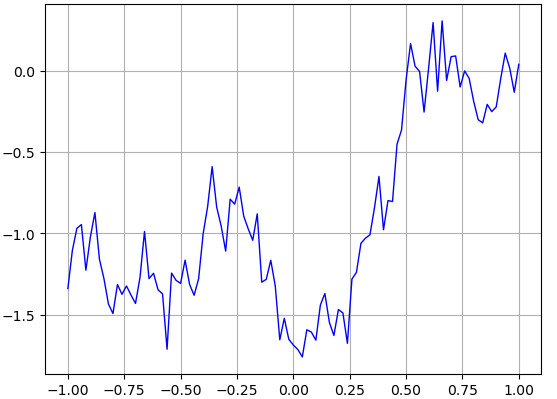
\includegraphics[scale=0.7]{images/gibbsRea.jpg}
\caption{Réalisation sur $[-1,1]$ par Galli-Gao-Gibbs}
\label{figGibbsRea}  
\end{center}
\end{figure}

\begin{remark}
  \label{nbIterationsMax}
  Dans OpenTURNS, l'algorithme se veut un peu différent en décidant pour une itération non pas de choisir un
  élément $a \in \llbracket 1;r \rrbracket $ selon une loi uniforme mais de tirer une permutation $\sigma$ de
  $\llbracket 1;r \rrbracket$ selon une loi uniforme puis de faire $r$ itérations où $a$ vaut d'abord $\sigma(1)$,
  puis $\sigma(2)$ jusqu'à $\sigma(r)$. Donc dans OpenTURNS, le nombre d'itérations $N_{it}$ mis en paramètre
  correspond dans les faits à $r \cdot N_{it} $ itérations où $r$ est la taille du vecteur gaussien à simuler.
\end{remark}

\section{Complexité algorithmique}
L'algorithme~\ref{algo5} admet une complexité en temps en
$O(Nr)$ et une complexité en mémoire en $O(r)$
(le stockage par des listes $z^n, z^c$ pour la simulation). Par
contre, pour l'algorithme~\ref{algo5} version OpenTURNS, en se fiant à la
remarque~\ref{nbIterationsMax}, bien que la complexité en mémoire reste inchangée,
la complexité en temps est en $O(N_{it}r^2)$ (pour une itération, lorsque $a$ parcourt
les valeurs de la permutation $\sigma$, $O(r)$ opérations
sont effectuées à chaque fois).

\section{Erreur et convergence numérique}
\label{gggErrConv}

\subsection{Dimension n=1}
Comme pour la méthode de Cholesky et celle des $\mathcal{H}$-matrices, pour simuler on a besoin 
d'un maillage $M$ et d'une fonction de covariance $C$ pour déduire $\Sigma$, la matrice de
covariance du problème $\Sigma$. Le choix des maillages et des fonctions de covariance sera celui
des maillages de la dimension $n=1$ évoqués pour la méthode de Cholesky (voir la sous-section~\ref{dimUnChol} du chapitre~\ref{chapCholesky})
et le nombre $m$ de n\oe uds dans les maillages ne variera plus entre $10$ et $10000$
mais plutôt entre $10$ et $100$ (pour des raisons de temps de calcul). Pour appliquer
la méthode de Galli-Gao-Gibbs, il faut aussi calibrer le nombre d'itérations $N_{it}$ évoqué à la
remarque~\ref{nbIterationsMax}. On décidera de le faire varier entre $10$ et $300$ pour les tests.


\subsection{Benckmarks}
\begin{table}[htbp]
  \centering
\begin{tabular}{|>{\centering\arraybackslash}p{1.5cm} |>{\centering\arraybackslash}p{1.6cm} |>{\centering\arraybackslash}p{1.0cm} |>{\centering\arraybackslash}p{2.0cm}|}
\hline
\small{Dimension } & \small{Nb de n\oe uds} & \small{$N_{it}$} & \small{Temps moyen d'une réalisation (en secondes)}\\
\hline
1 & 10 & 100 & 0.00637s    \\
\hline
1 & 10 & 200 & 0.01468s  \\
\hline
1 & 10 & 300 & 0.02217s   \\
\hline
\hline
1 & 100 & 100 & 0.15972s    \\
\hline
1 & 100 & 200 & 0.34042s    \\
\hline
1 & 100 & 300 & 0.47059s    \\
\hline
\end{tabular}
\end{table}

\begin{table}[htbp]
  \centering
\begin{tabular}{|c |c |c |c |c |}
\hline
Dimension & Nb de n\oe uds & $N_{it}$ & Nb de réalisations & erreur $L^2$ \\
\hline
1 & 10 & 10 & 250 & 0.18609  \\
\hline
1 & 10 & 10 & 500 & 0.11308   \\
\hline
1 & 10 & 10 & 750 & 0.07441  \\
\hline
1 & 10 & 10 & 1000 & 0.07942 \\
\hline
\hline
1 & 10 & 50 & 250 & 0.17034 \\
\hline
1 & 10 & 50 & 500 & 0.12572  \\
\hline
1 & 10 & 50 & 750 & 0.08582  \\
\hline
1 & 10 & 50 & 1000 & 0.08190 \\
\hline
\hline
1 & 10 & 100 & 250  & 0.14295 \\
\hline
1 & 10 & 100 & 500  & 0.10940 \\
\hline
1 & 10 & 100 & 750  & 0.09015  \\
\hline
1 & 10 & 100 & 1000 & 0.06226  \\
\hline
\hline
1 & 100 & 10 & 250 & 0.25851  \\
\hline
1 & 100 & 10 & 500 & 0.19295   \\
\hline
1 & 100 & 10 & 750 & 0.15731  \\
\hline
1 & 100 & 10 & 1000 & 0.13206 \\
\hline
\hline
1 & 100 & 50 & 250 & 0.27869 \\
\hline
1 & 100 & 50 & 500 & 0.18906  \\
\hline
1 & 100 & 50 & 750 &  0.16029 \\
\hline
1 & 100 & 50 & 1000 & 0.13728 \\
\hline
\hline
1 & 100 & 100 & 250  & 0.30028 \\
\hline
1 & 100 & 100 & 500  & 0.18475 \\
\hline
1 & 100 & 100 & 750  & 0.14346  \\
\hline
1 & 100 & 100 & 1000 & 0.13889  \\
\hline
\end{tabular}
\end{table}
